\subsection{Szűrők - elméleti áttekintés}

Szűrés által csillapítani (kiszűrni) tudjuk a jelekből a nem kívánt frekvencia komponenseket úgy, hogy a számunkra fontos frekvencia komponenseket változatlanul átengedjük.

\subsection{Átviteli függvény}

Egy szűrőt megadhatunk egy átviteli függvény segítségével. Az átviteli függvény adja meg a rendszer kimenetei és bemenetei közötti összefüggést. 

A szűrés történhet úgy, hogy a jelet átvisszük a frekvencia tartományba (Fourier transzformált), összeszorozzuk az átviteli függvénnyel és ezután visszavisszük az időtartományba (Inverz Fourier transzformált). Egy másik lehetőség (FIR szűrő), hogy az átviteli függvénynek elvégezzük az inverz Fourier transzformáltját, így a szűrés csak egy egyszerű konvolúció a bemeneti jel és a súlyfüggvény között (a frekvencia tartományban szorzás megfelel az időtartományban a konvolúcióval).

\subsection{Szűrő struktúrák}

Több fajta szűrő létezik:

\begin{itemize}
    \item Alul-áteresztő
    \item Felül-áteresztő
    \item Sávzáró
    \item Sáváteresztő
    \item Mindent áteresztő (fázist változtatja meg, például sztereó hangzás eléréséért)
\end{itemize}

\begin{figure}[H]
    \centering
    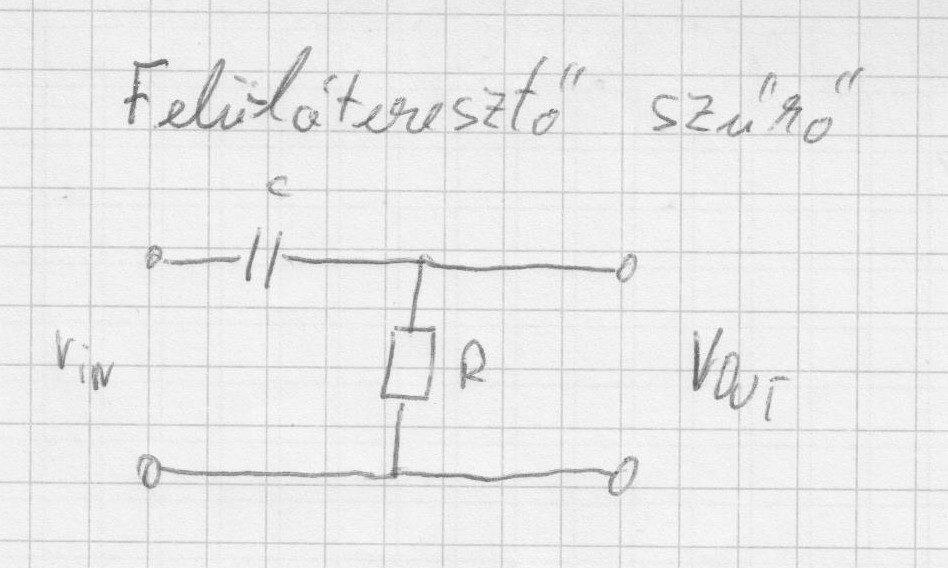
\includegraphics[scale=0.25]{figures/szuro_hp_rc.jpg}
    \caption{Felül-áteresztő szűrő}
\end{figure}

\begin{figure}[H]
    \centering
    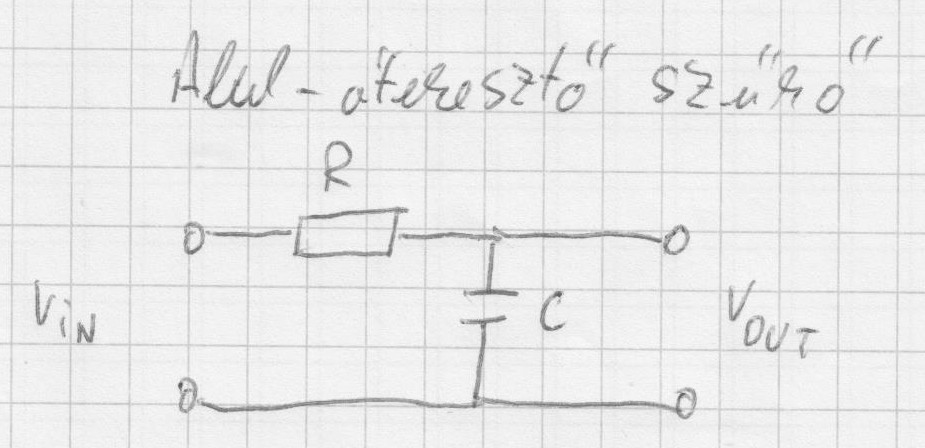
\includegraphics[scale=0.25]{figures/szuro_lp_rc.jpg}
    \caption{Alul-áteresztő szűrő}
\end{figure}

\subsection{Frekvencia, amplitúdó és fáziskarakterisztikák}

Frekvencia karakterisztikák: áteresztő tartománybeli erősítés ingadozás, átmeneti tartomány meredeksége, zárótartományi csillapítás ingadozás.

\begin{figure}[H]
    \centering
    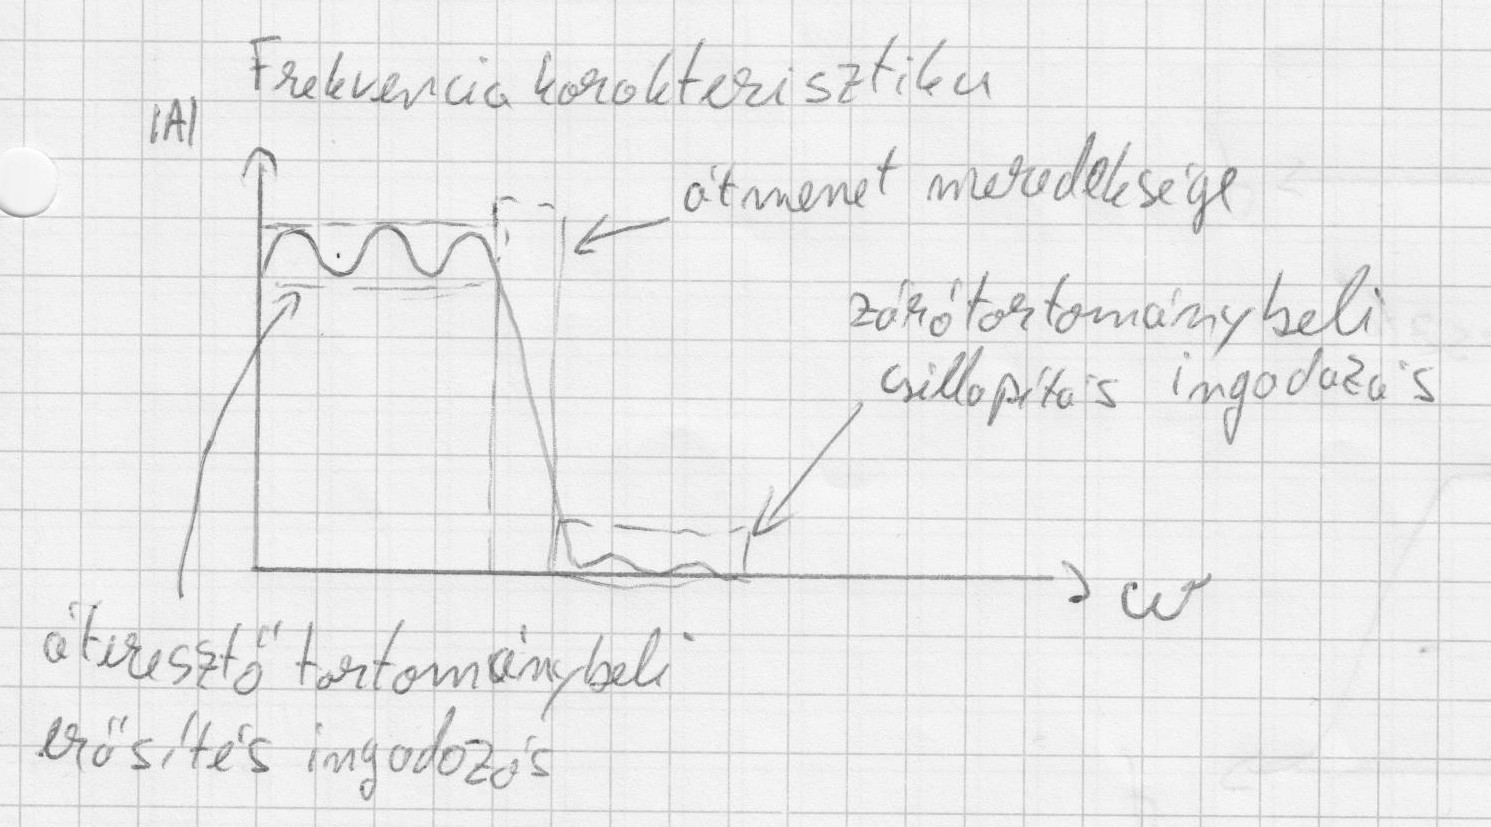
\includegraphics[scale=0.25]{figures/szuro_frekv.jpg}
    \caption{Frekvenciakarakterisztika}
\end{figure}

Fáziskarakterisztikák: fázismenet, csoportfutási idő. Fázismenet lehet lineáris vagy nemlineáris. Lineáris esetén minden frekvenciakomponenst ugyanannyit késleltet a szűrő. A csoportfutási idő a fázismenet frekvencia szerinti deriváltja.

\begin{figure}[H]
    \centering
    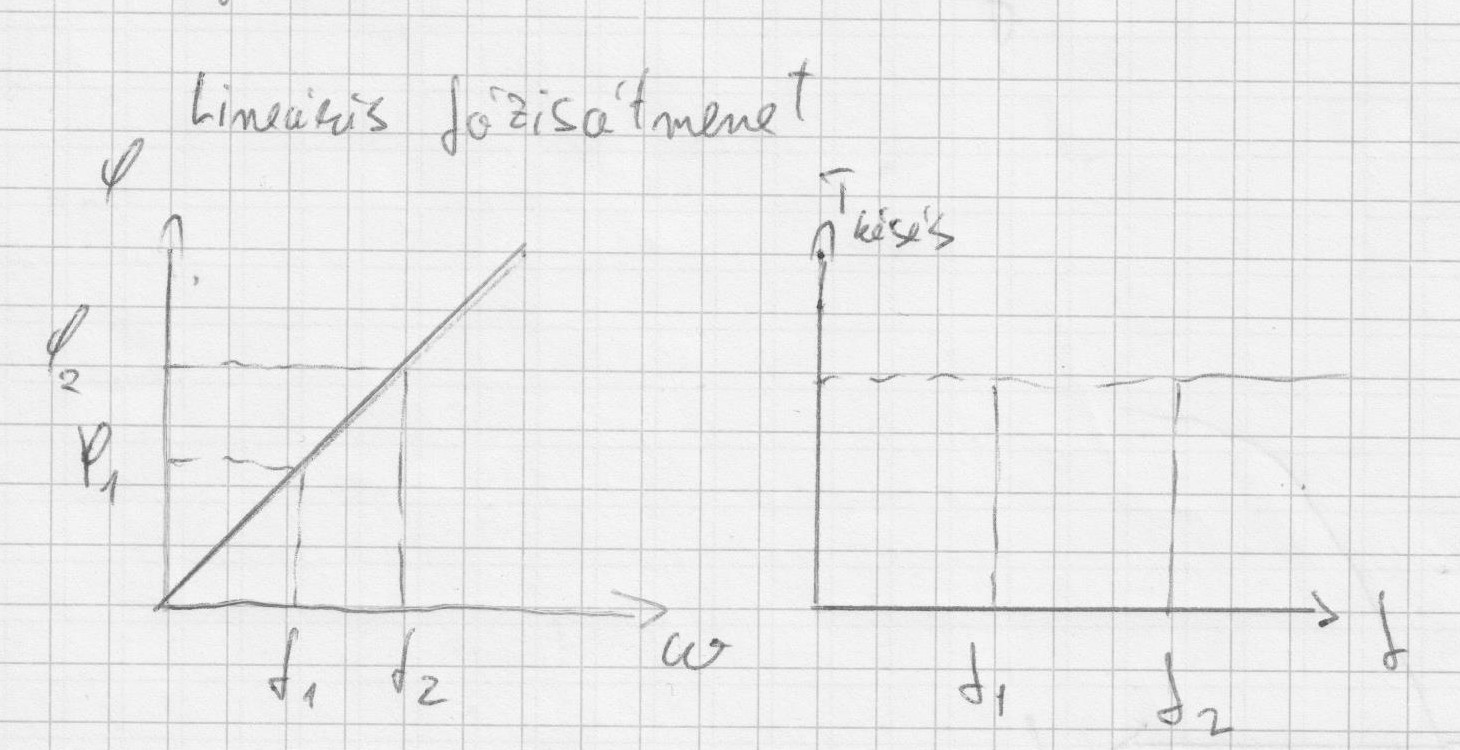
\includegraphics[scale=0.25]{figures/szuro_lin_menet.jpg}
    \caption{Lineáris fázismenet}
\end{figure}

\begin{figure}[H]
    \centering
    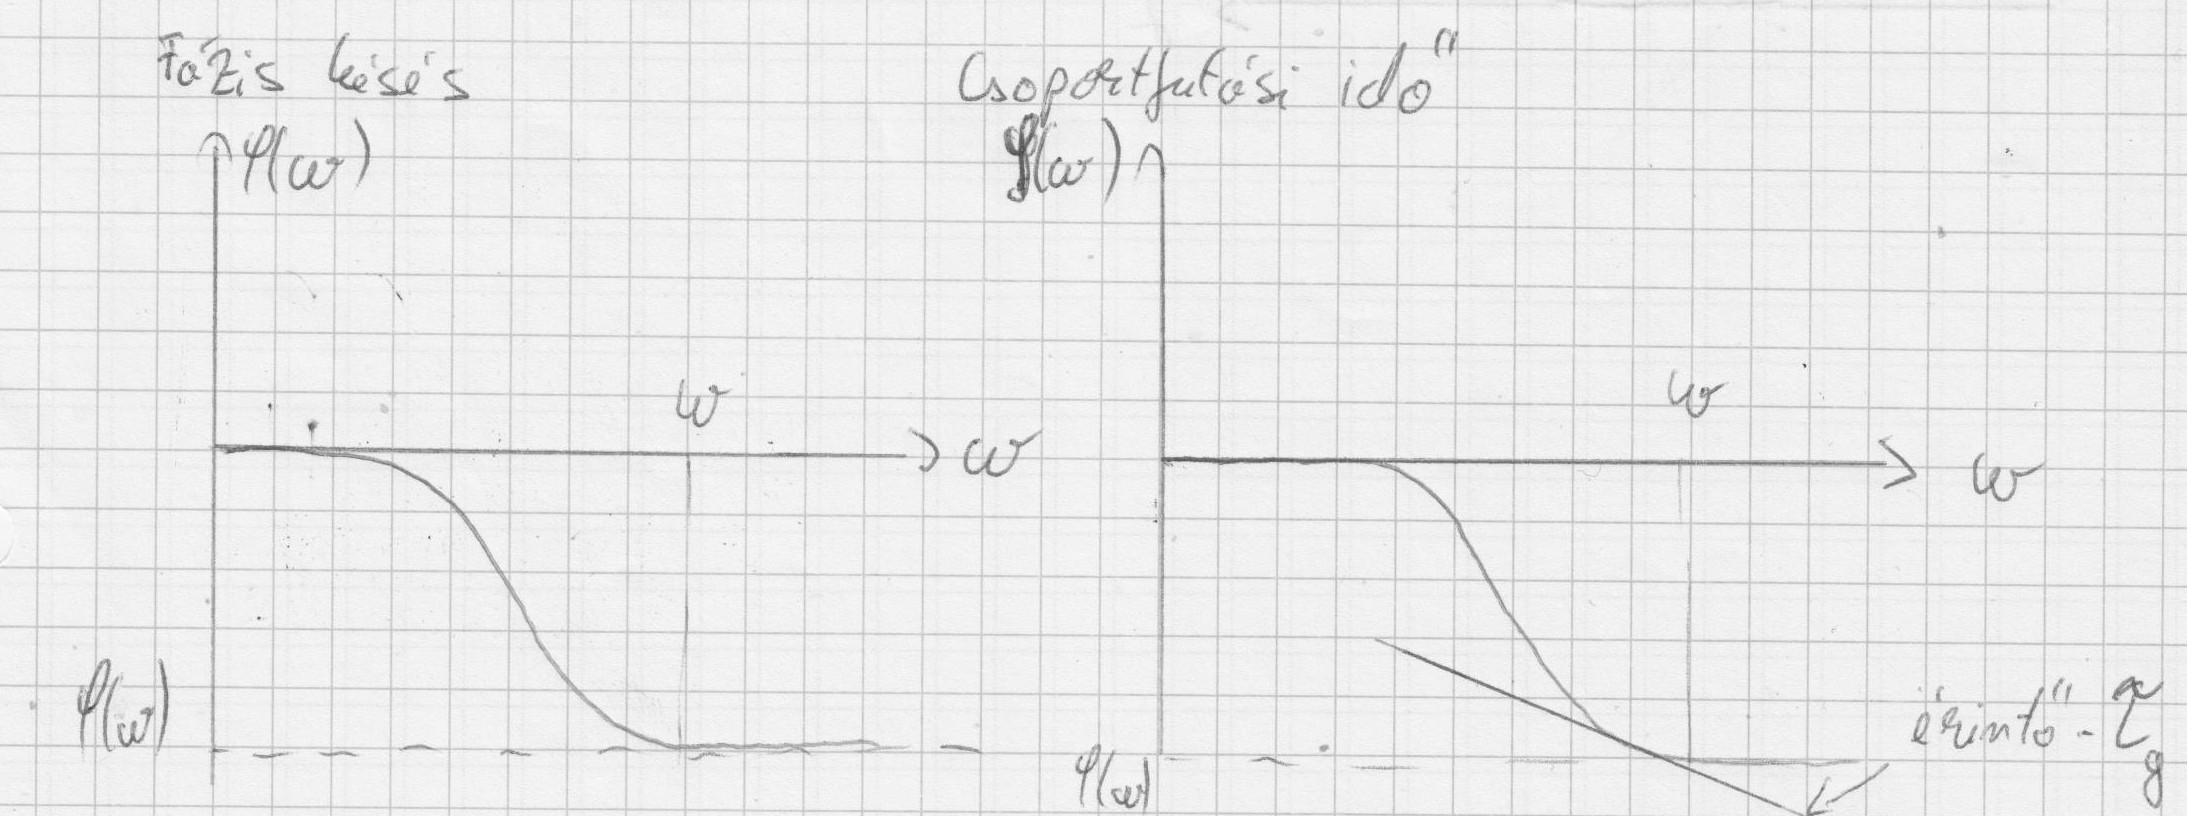
\includegraphics[scale=0.20]{figures/szuro_faz_csoport.jpg}
    \caption{Fáziskésés és csoportfutási idő}
\end{figure}

\begin{itemize}
    \item Fáziskésés: $\tau_{p}(w) = \frac{\varphi(w)}{w} $
    \item Csoportfutási idő: $\tau_{g}=\frac{d\varphi(w)}{dw}$
\end{itemize}


\subsection{Szűrő válaszának skálázása}

Az analóg szűrőknek az átviteli függvényük $f_{c} = 1$-re vannak normalizálva. Ahhoz, hogy a kívánt frekvenciánál legyen a vágás, szükséges, hogy a következő képlet szerint számoljuk ki az átviteli függvényt: $H_{w_{c}}(s) = \frac{k * \Pi_{i=1}^{n}(s - w_{c} * z_{i})}{w_{c}^{m - n} \Pi_{j=1}^{n} (s - w_{c}*p_{j})}$

\begin{itemize}
    \item $w_{c}$: vágási körfrekvencia
    \item $k$: erősítés
    \item $z_{i}$: zérusok
    \item $p_{j}$: pólusok
\end{itemize}

\subsection{Ábrázolási módok}

Hasznos az ábrázolási módot úgy végezni, hogy az áteresztőtartományban lineáris a skála (nagy felbontás), és a zárótartományban logaritmikus. Frekvencia tartományban ábrázoljuk a szűrőket, mert ott látható, hogy a szűrő melyik frekvenciákat engedi át és melyikeket nem.

\subsection{Szűrőtípusok közötti transzformációk}

Egy jól megtervezett alul-áteresztő szűrőből egy behelyettesítés elvégzése által lehet felül-áteresztő, sáváteresztő és sávzáró szűrőt kapni.

Felül-áteresztő: $H_{FE}: s \rightarrow \frac{1}{s}$

\begin{figure}[H]
    \centering
    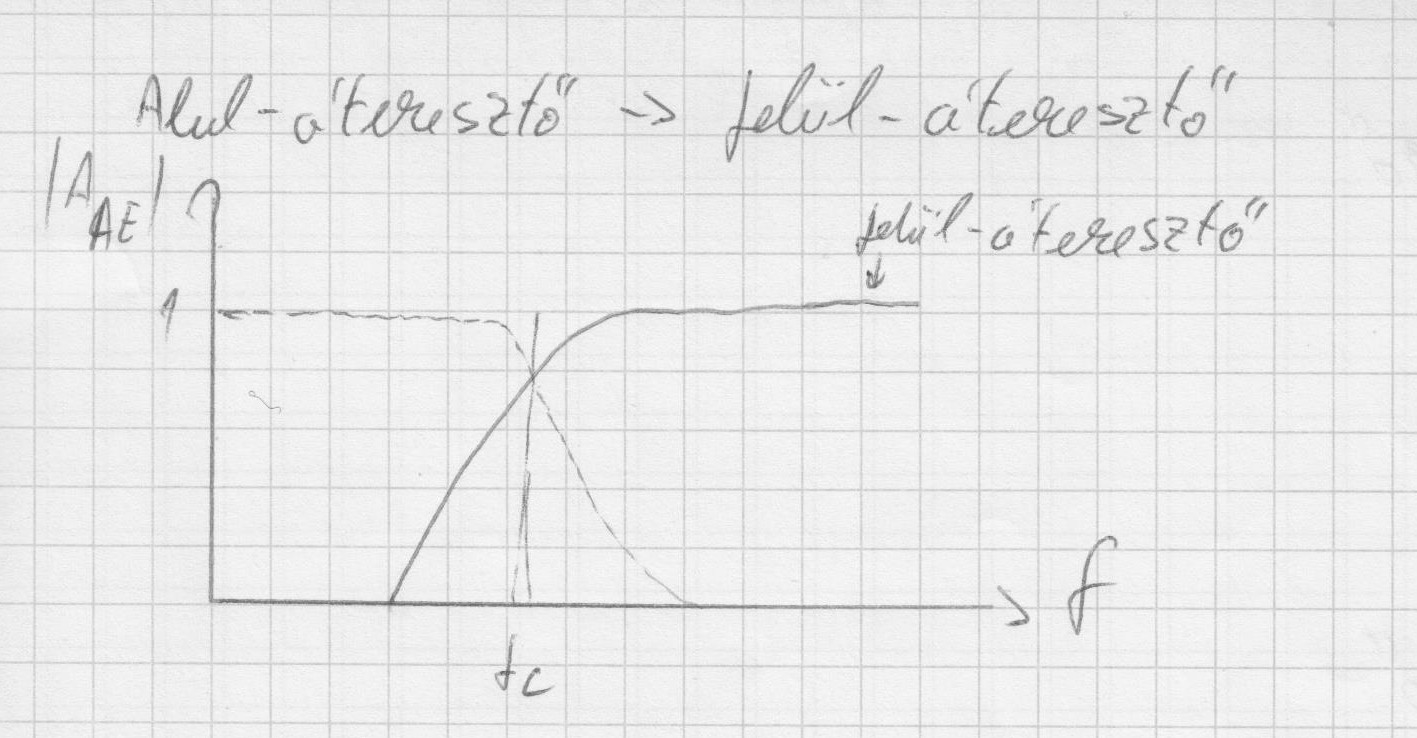
\includegraphics[scale=0.2]{figures/szuro_hp.jpg}
    \caption{Felül-áteresztő szűrő}
\end{figure}

Keskeny sávú sáváteresztő: $H_{SA}: s \rightarrow s - \frac{1}{s}$

\begin{figure}[H]
    \centering
    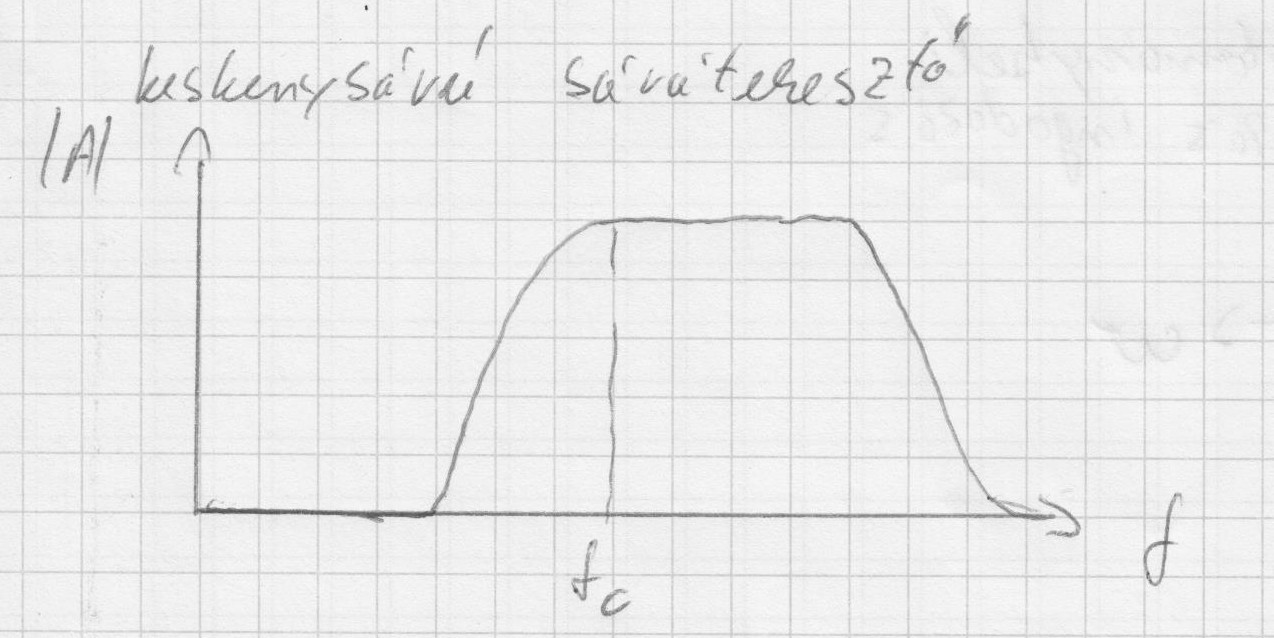
\includegraphics[scale=0.2]{figures/szuro_bp_good.jpg}
    \caption{Keskeny sávú sáváteresztő}
\end{figure}

Sáváteresztőt lehet egy alul-áteresztő és felül-áteresztő szűrő egymás utáni kapcsolásával is megvalósítani. Ez viszont behoz egy nem kívánt csillapítást az áteresztő tartományban.

\begin{figure}[H]
    \centering
    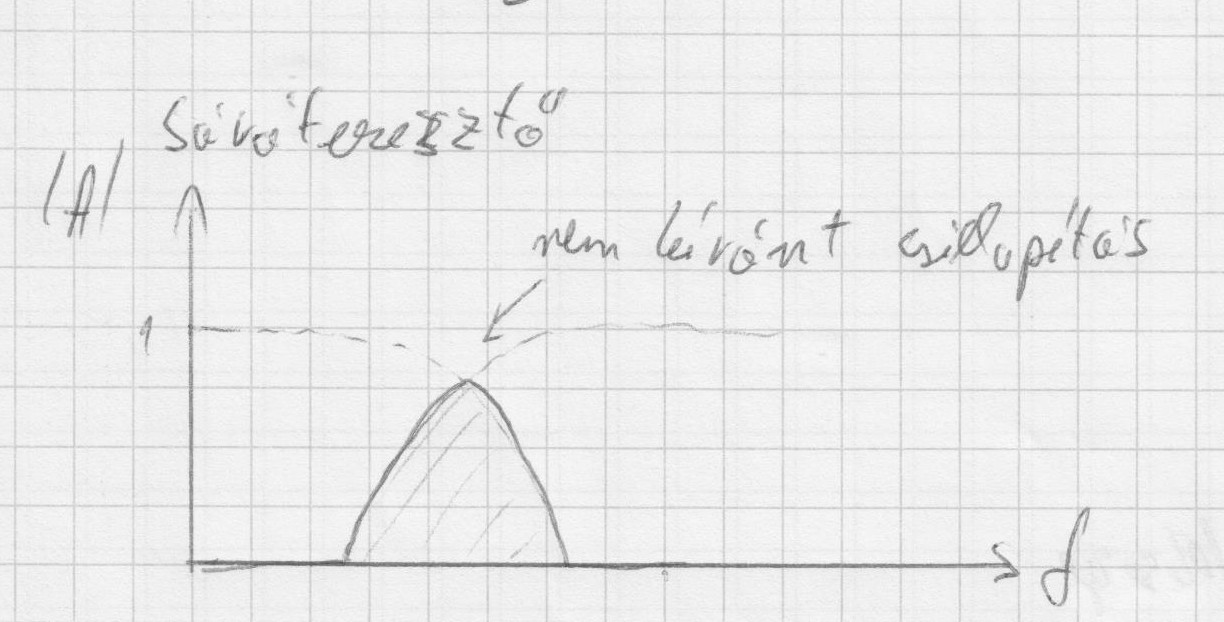
\includegraphics[scale=0.2]{figures/szuro_bp.jpg}
    \caption{Sáváteresztő: AE + FE szűrő kapcsolás}
\end{figure}

Sávzáró: $H_{SZ}: s \rightarrow \frac{s}{s^{2} - 1}$

\begin{figure}[H]
    \centering
    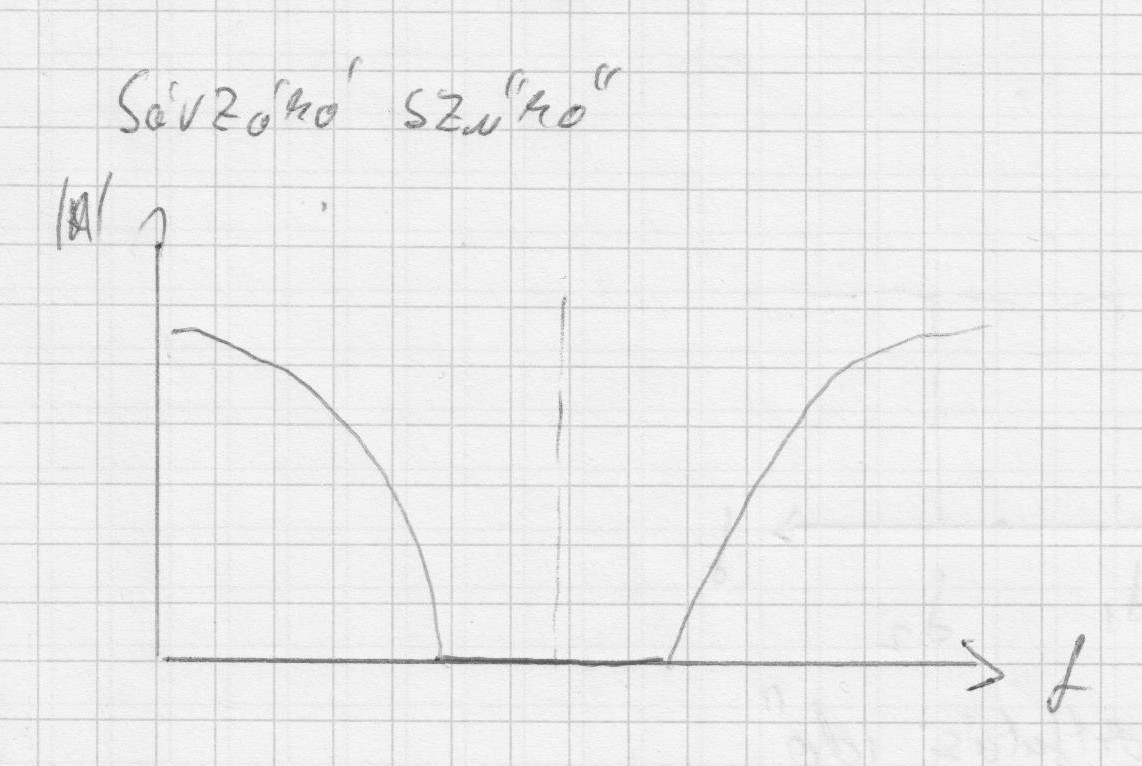
\includegraphics[scale=0.2]{figures/szuro_bs.jpg}
    \caption{Sávzáró szűrő}
\end{figure}
